%Research Plan - 20%
\section{Research Plan} 
\label{sec:research}

Given the ever-growing flood of information, Cartography provide an visually appealing way to present the world reality. The approach of this project is to visualize covid cases among different states of Northern America on the basis of per capita using cartographic mapping. 
The visualization of the covid pandemic can be classified as two types, static visualization \cite{WaPo} and complex interactive visualization \cite{CovViz} which gives overall perspective but hinder to provide details required for the user  to go in deep for the particular region and how the region is affected. This project aims to include interactive visualization and provide details of each region in the northern America on the basis of proportional statistics ie; there will be clear distinction between the severity or improvement in cases based on universal scaling and on the other hand calculating the number of cases based on total number of people in the region. 
According to work presented by Zhou et al. \cite{Zhou}, they categorize “visualization technique” as low level operation and “visual task” as interface between the visual representation and visual techniques without specifying “how” an operation is done. This project aims to facilitate both these categorization by implementing cartography based on two components such as population of each state and different metrics of covid cases in each state. In order to show the metrics such as positive cases, negative cases, total tests, recovery cases and number of death from covid in each state, we have included the mouse hover effect interaction through which, by hovering over the states, we can show details of all the metrics of the respective state. Sequential color scheme has been implemented to forecast the impact of covid and changes as per naïve data and per capita data for each metric. This project is implemented using interactive visualization for mouseover, click, mouseout and button based interactions.

\begin{figure}[h]
 \centering % avoid the use of \begin{center}...\end{center} and use \centering instead (more compact)
 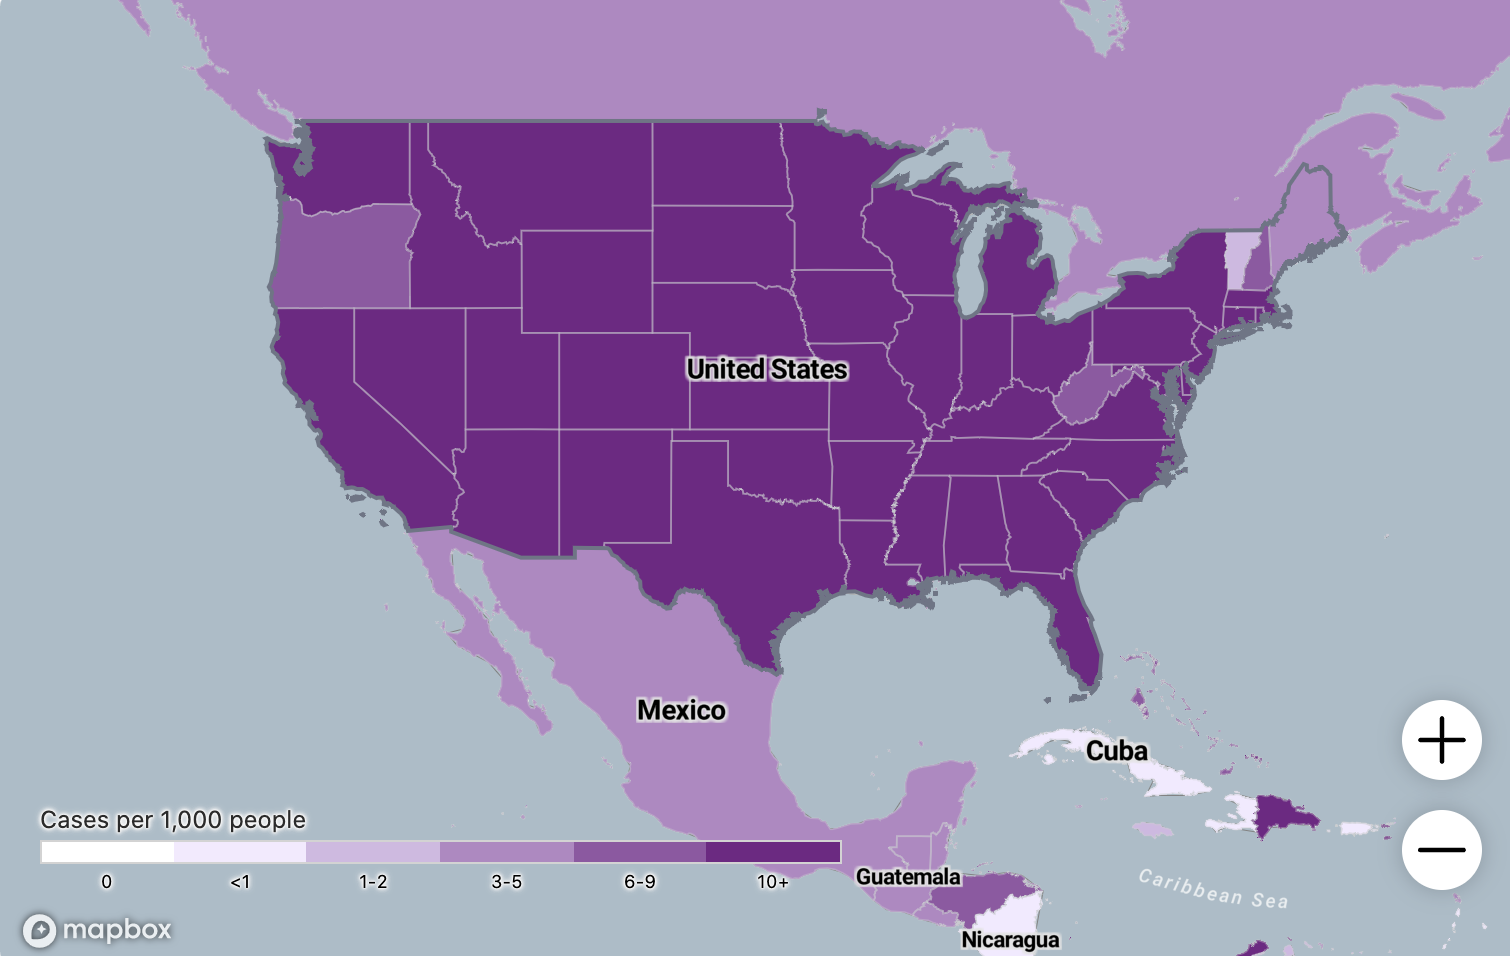
\includegraphics[width=3in]{figs/Weatherdata.png}
 \caption{Choropleth map for weather data \cite{Weather}}
 \label{fig:weather}
\end{figure}

\subsection{Data}
\label{sec:data}

Data for this project is taken from the COVID Tracking Project \cite{CTP}. This dataset includes the latest Covid-19 statistics from March till date and is updated daily. The data is categorized state-wise and shows different parameters including number of positive cases, number of negative cases etc. Population data of USA has been taken from a reference lookup table \cite{PopData}. This dataset includes total population of the country and categorized from highest to lowest as per state according to the population. 

\subsection{Evaluation}
\label{sec:eval}

The project can be evaluated on the basis of the milestones as shown in the timeline section. Some metrics for evaluation can be – efficacy of the cartographic mapping technique in showing the covid spread, the correlation plots between different categories and the implementation of additional features like mousein, mouseout, zoom etc.
Another metric is to evaluate the flexibility of the implemented visualization technique to handle changes in data since the data can change quite quickly. The visualization technique has to ensure that overcrowding doesn’t happen due to the saturation of datapoints and this becomes a key metric to ensure the data is well presented.

\subsection{Technology}
\label{sec:tech}

As D3 \cite{d3js} supports web mapping and interaction and also supports topology projection. This project will be implemented using d3.js and HTML5 and Using Topojson library \cite{top} to encode the topology. 
Above mentioned list of technologies are extremely powerful when it comes for handling geographical information. 

\subsection{Results}
\label{sec:Prelim}
Following is the list of updates on the implementation :
\begin{itemize}
\item Data has been taken from The Covid Tracking project and choropleth map has been implemented in d3.v5. The data only contains statewide information and does not have county-wise split-up. Hence, the choropleth map shows the color coding for positive cases (by default) based on states.
\item Cumulative plots are added where clicking on any state will show the Covid trend in each state – 5 different plots are shown for the different metrics like number of positive, negative, total tests, total recovered and number of deaths. It is possible to compare data between states by clicking on different states. Double clicking on the map clears all the plots.
\item Buttons are added to switch the data being displayed to negative cases, total number of recovered, number of tests etc. The color coding changes based on the data being displayed along with the legend scale.
\item Hovering over the states (mouseover) brings up a pop-up showing the details for the particular state. This includes the data for the latest date (two days prior data is chosen as latest date to allow time for data to be uploaded fully).
\item State and county borders are shown though county information is not processed. Handling county information needs input from different sources. This can be tricky since data may not correlate exactly between different sources.
\item Two lookup tables are used in this project – One (lookup.csv) to generate the population data for different states [cite] (in order to calculate the per Capita information) and the second one (stateLookup.csv) to map fips codes to state code and the state names.
\item In order to read json and csv files, since the browser does not allow accessing local files, a local server had to be created following the steps shown in \cite{server}. The server was created using the web sever extension for Chrome. 
\end{itemize}

\par Fig \ref{fig:Implementation-1} shows the implementation of the choropleth map sequential color scheme(grey to red) to denote higher and lower cases of each metric.
\begin{figure}[h]
 \centering 
 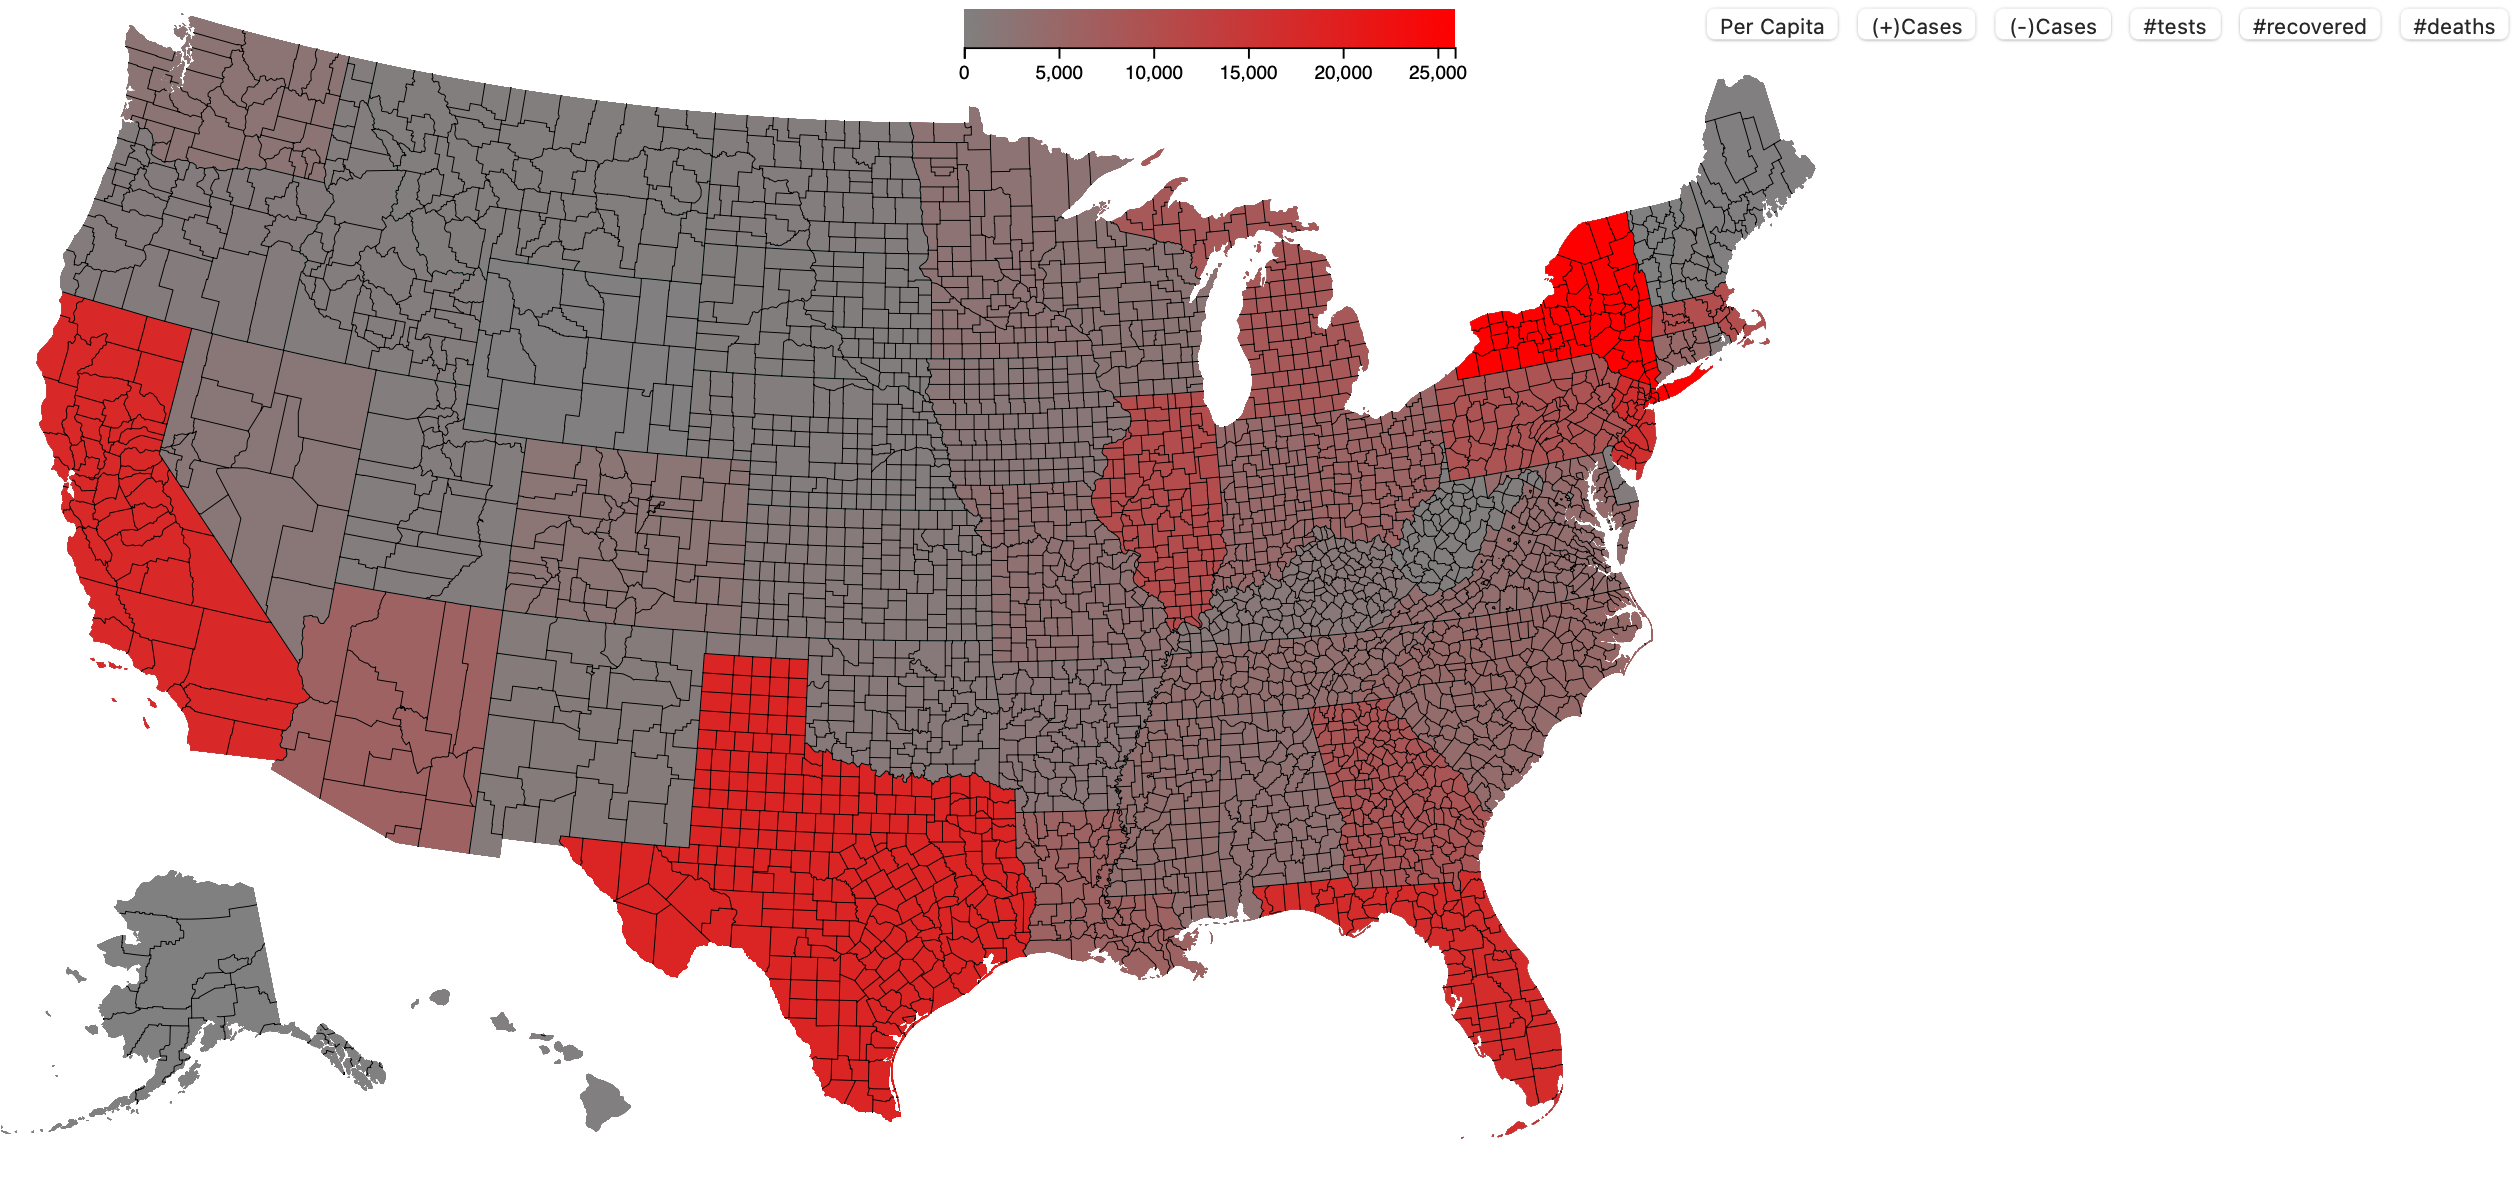
\includegraphics[width=3in]{figs/Implementation-1.png}
 \caption{Implemented choropleth map showing choropleth map sequential color scheme(grey to red)}
 \label{fig:Implementation-1}
\end{figure}

\par Fig \ref{fig:Implementation-2} shows mouseover showing the details for the other metrics considered like positive cases, negative cases etc.
\begin{figure}[h]
 \centering 
 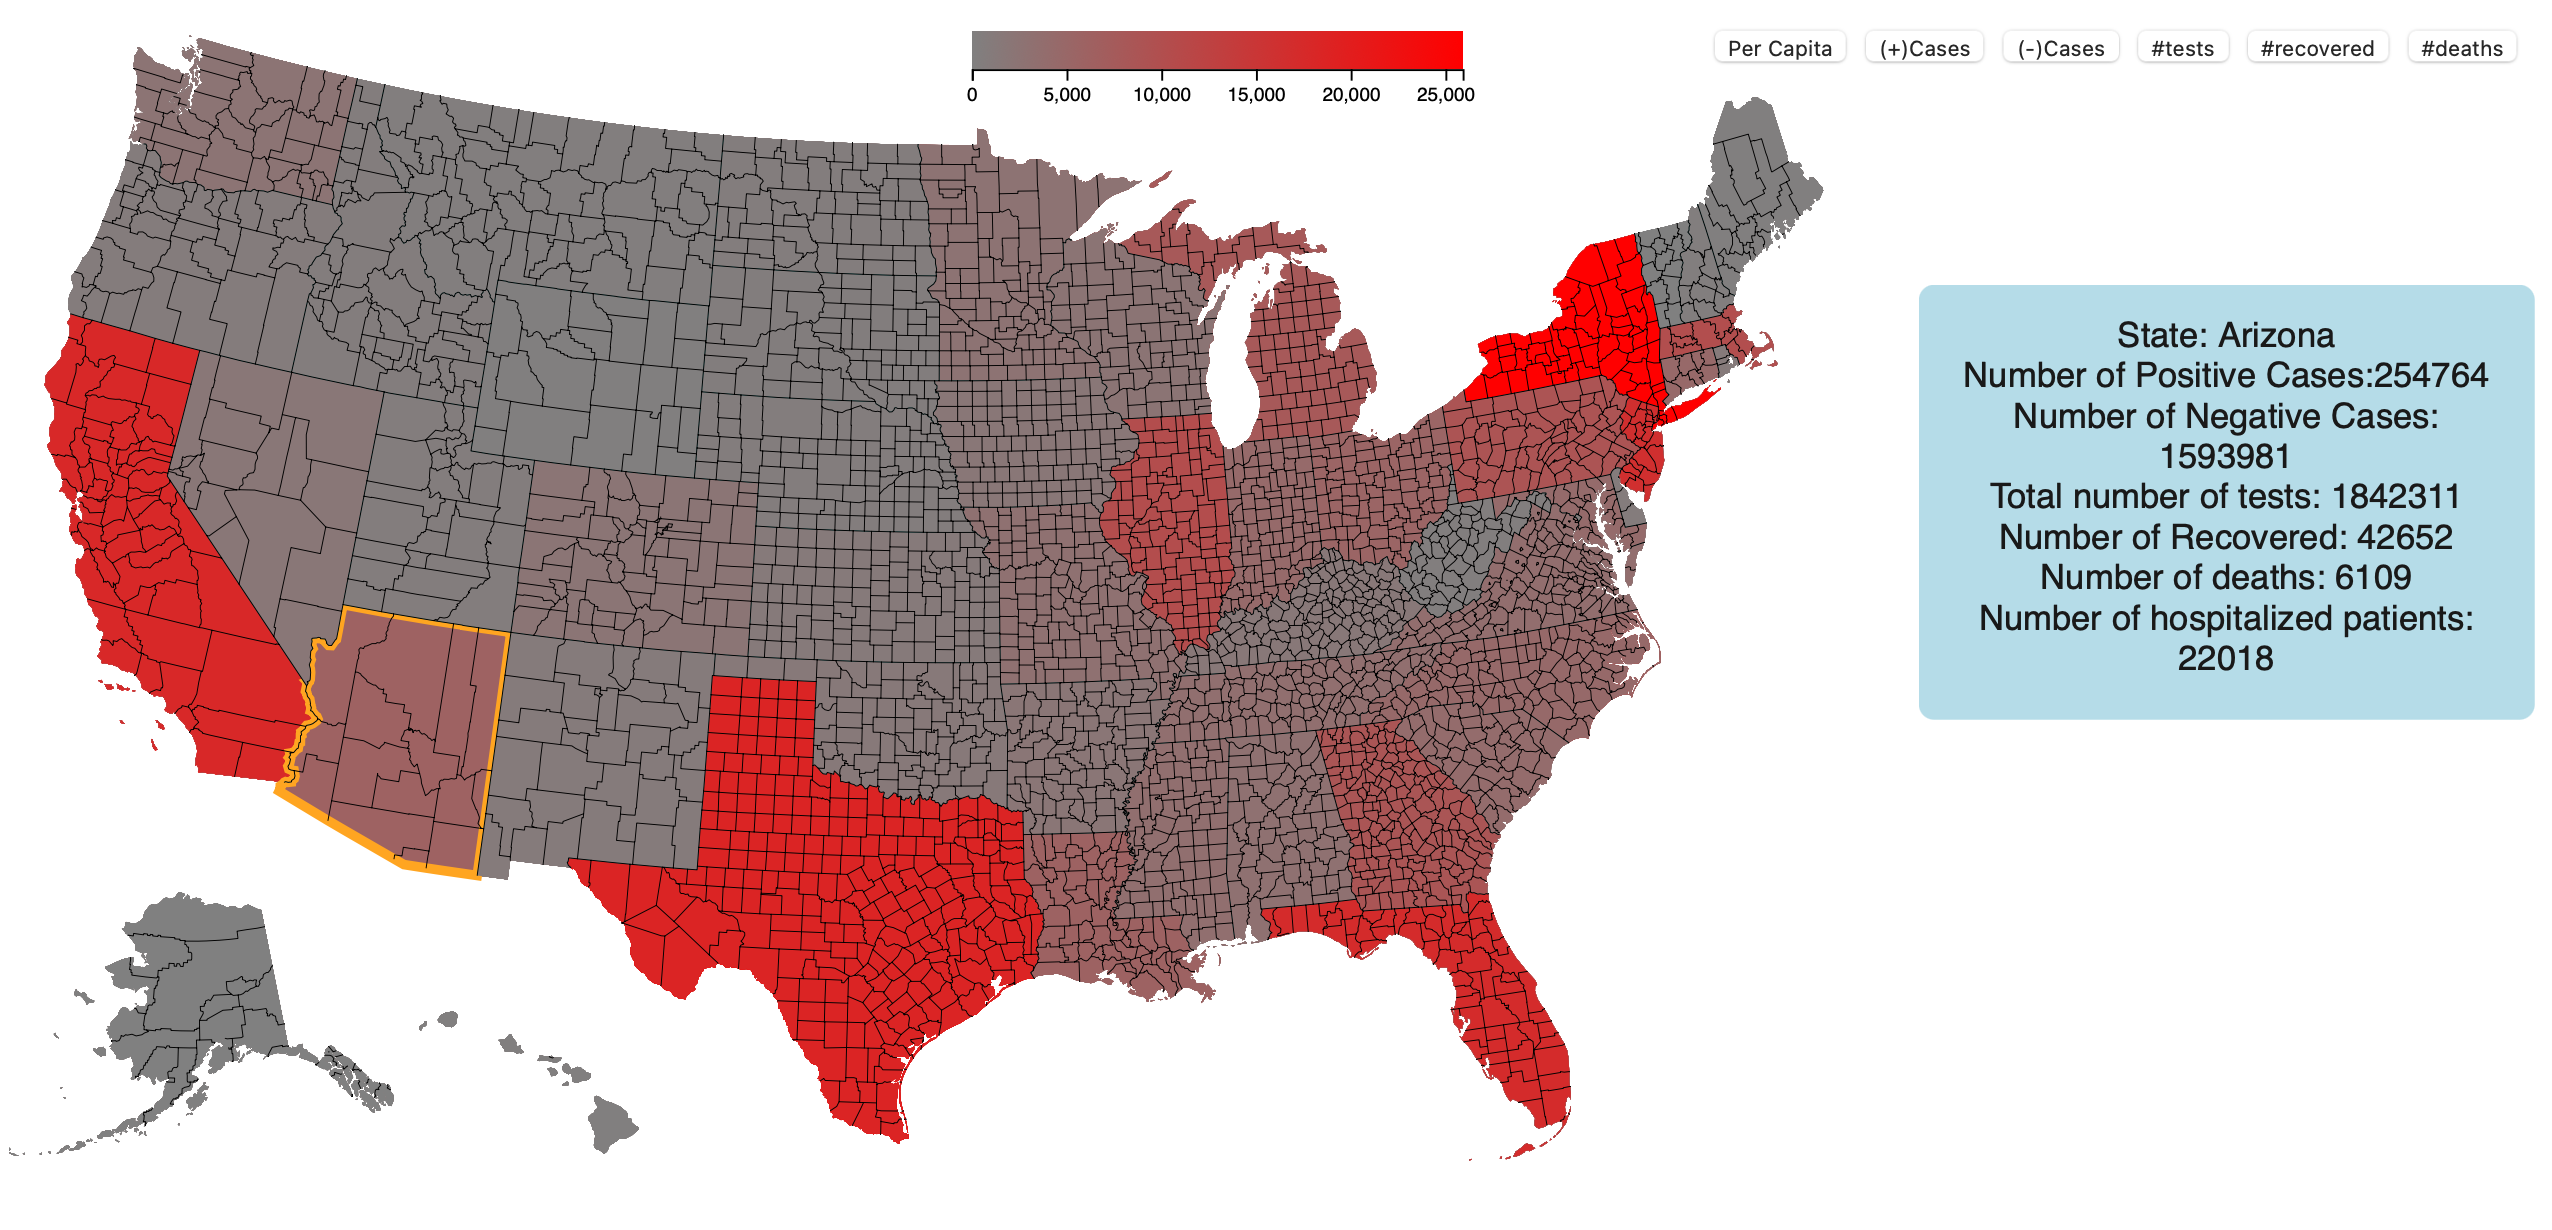
\includegraphics[width=3in]{figs/Implementation-2.png}
 \caption{Implemented choropleth map showing mouseover showing the details for the other metrics }
 \label{fig:Implementation-2}
\end{figure}

\par Fig \ref{fig:Implementation-3} shows the comparison data generated for two states by using the click function.
\begin{figure}[h]
 \centering 
 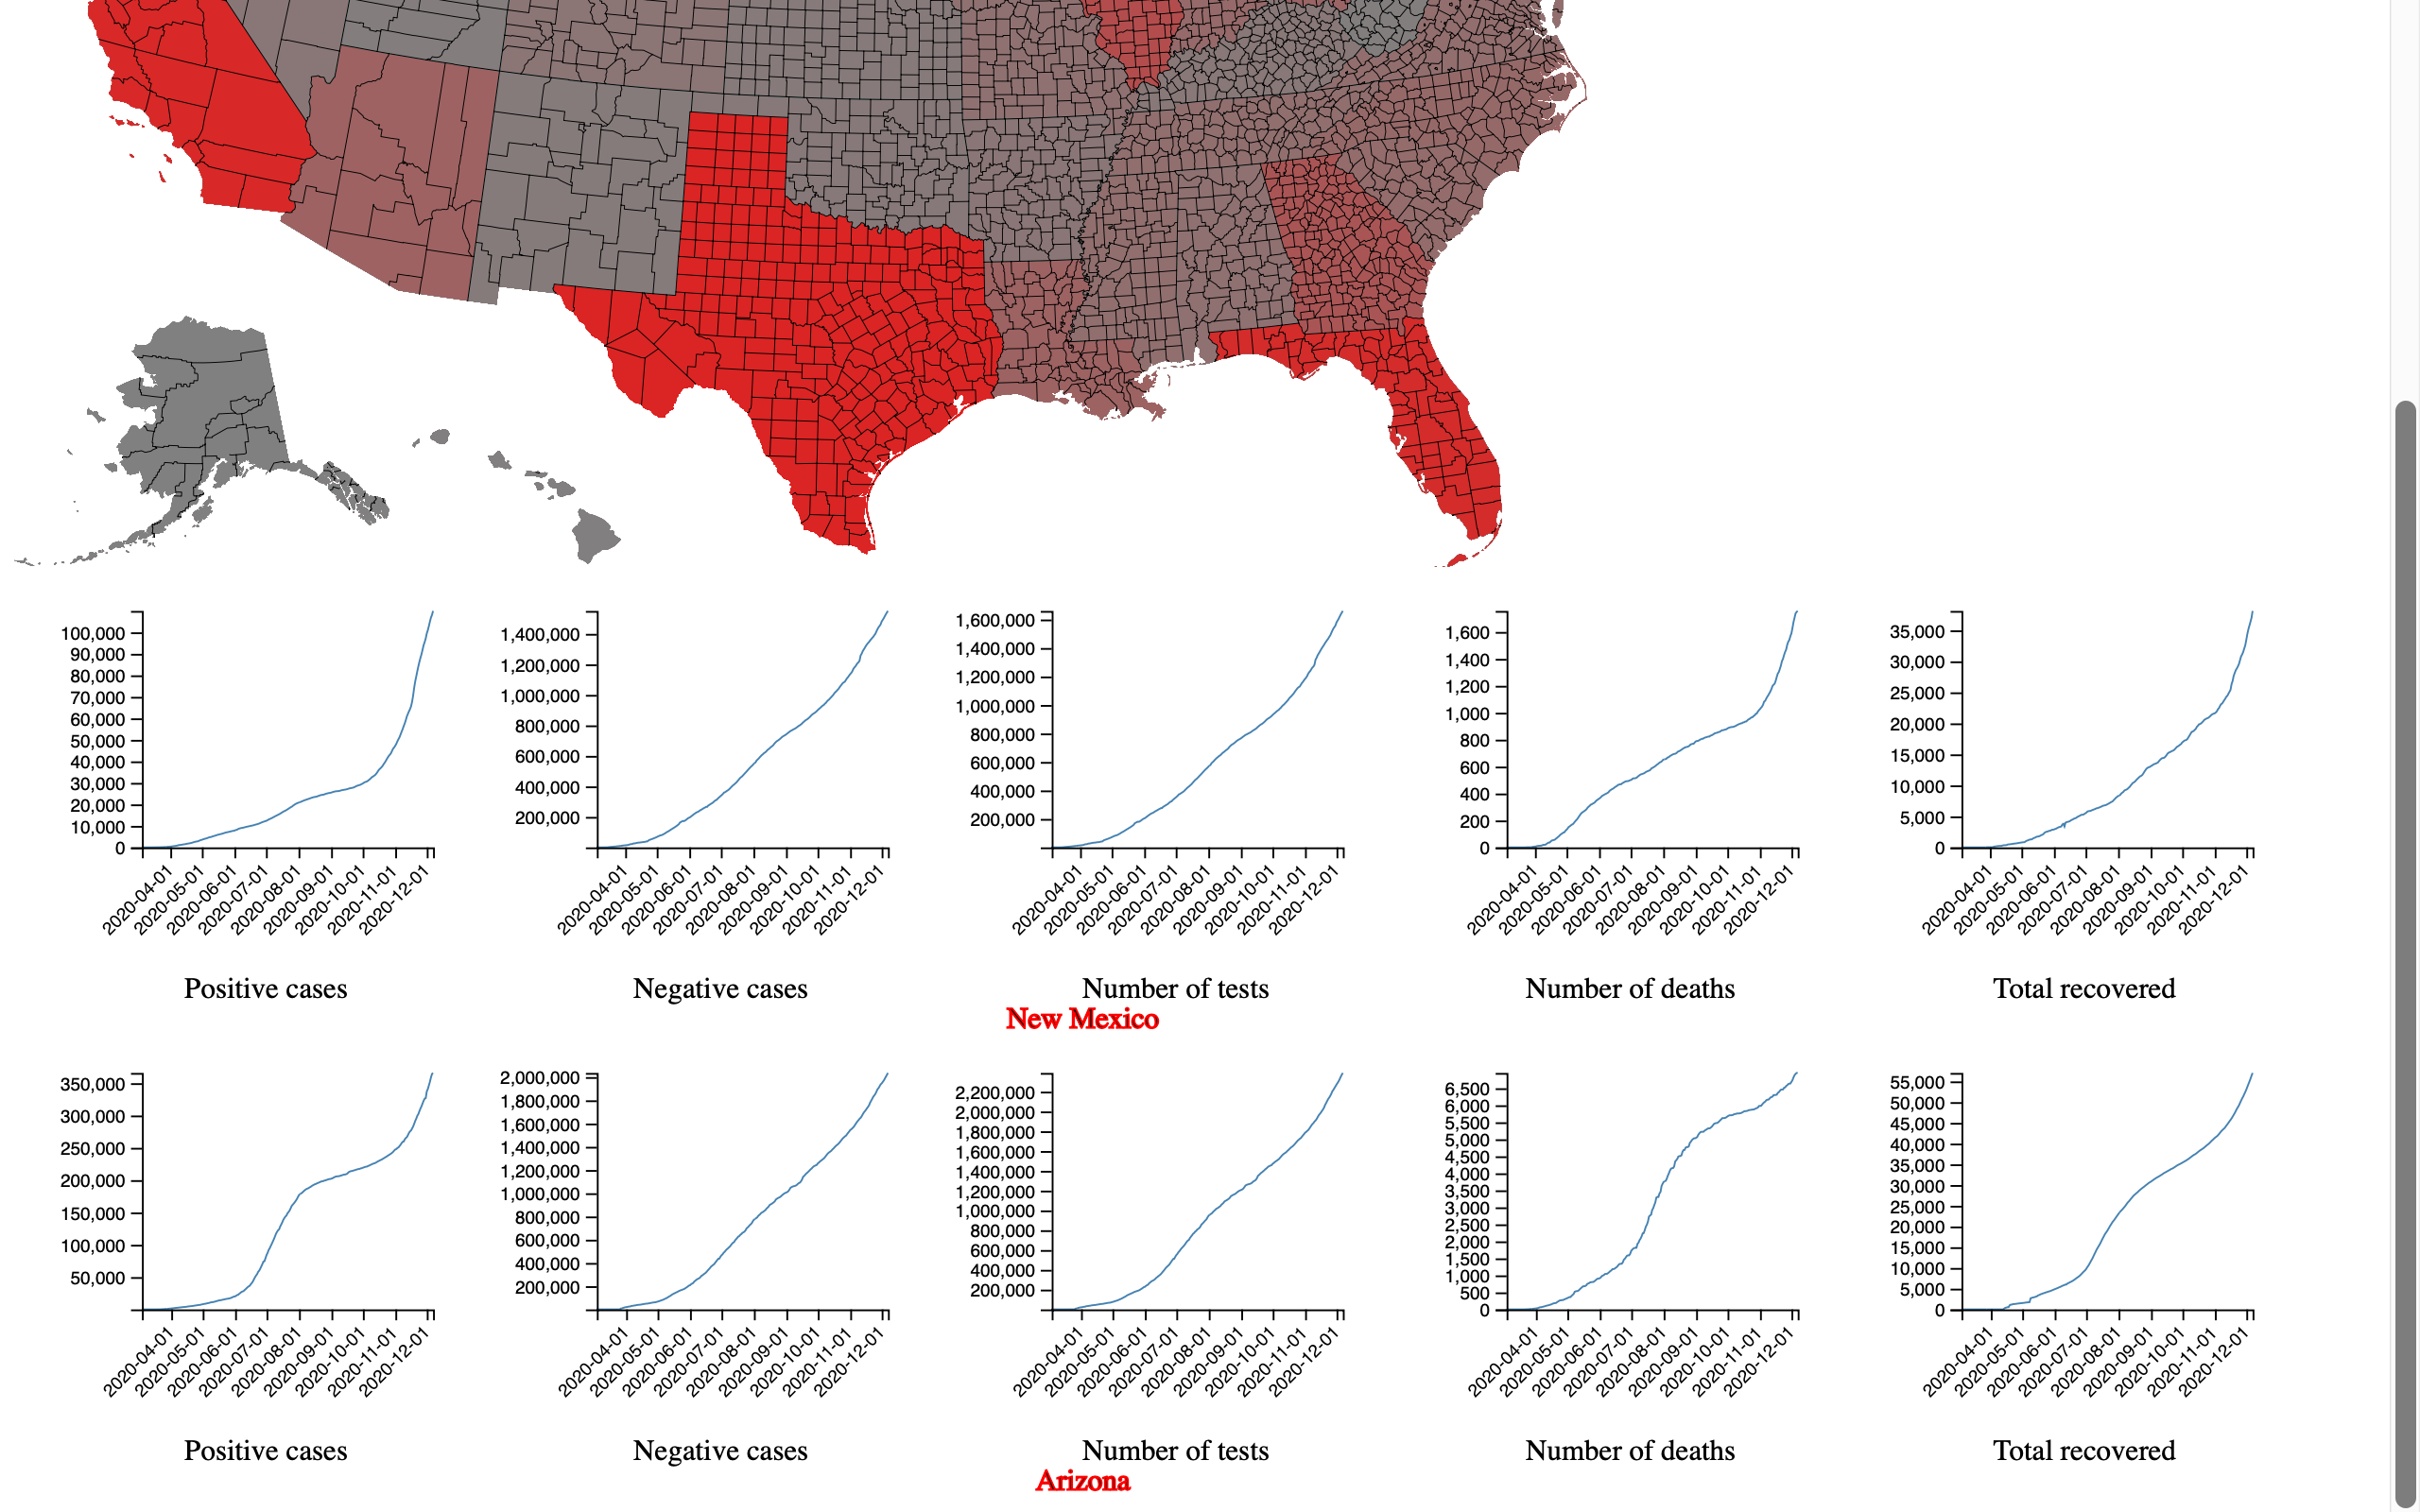
\includegraphics[width=3in]{figs/Implementation-3.png}
 \caption{Implemented choropleth map showing comparison data generated for two states by using the click function}
 \label{fig:Implementation-3}
\end{figure}



\subsection{Timeline}
\label{sec:timeline}

The milestones along with the description of what is achieved in each of them is shown below :

\paragraph{Milestone 1}
\begin{itemize}
\item Loaded the geographic dataset into Topojson format. The Topojson format helps in encoding geometric features such as point, line string, multiline string using coordinats that each of them feature.
\item Create SVG canvas for the map.
\end{itemize}

\paragraph{Milestone 2}

\begin{itemize}
\item Turned the Topojson data into screen co-ordinates using built-in projections in d3\cite{proj}.
\item To set up the path generator and its dimensions \cite{geoPath}.  This helps to generate the path data string as an attribute for SVG path element.
 \item Binding the data to SVG.
\item Progress Update
\item Added data to the map(by creating the g element and append the path element)
\item Added interactions to the map by using page elements to pop information on the map.(eg: adding page elements to display the count of covid cases in each state on the map)
\end{itemize}

\paragraph{Milestone 3}
\begin{itemize}
\item Added zoom on feature to make the visualization more interactive specially for north eastern states which are small to hover on.
\item Parsed the data more efficiently and having a lookup for multi-data handling.
\end{itemize}

\paragraph{Milestone 4}
\begin{itemize}
\item Added cumulative data instead of single date - to show choropleth map for the latest date and add onclick function to show progression from early on till date.
\item Compare statistics of any number of states by clicking on states and viewing the cumulative plots of each state which range from March to the current date.
\item Choropleth map is automatically updated to the latest date by extracting the latest data from the COVID Tracking Project to showcase latest trend of COVID spread.
\item Project report and documentation
\end{itemize}

\begin{table}[h]
%% Table captions on top in journal version
 \caption{Project Milestones}\vspace{1ex} % the \vspace adds some space after the top caption
 \label{tab:milestones}
 \scriptsize
 \centering % avoid the use of \begin{center}...\end{center} and use \centering instead (more compact)
   \begin{tabular}{r|r}
     Milestone & Description\\
   \hline
     Oct 15 & Load dataset  \\
     Oct 29 & Adding data to map \\
Nov 15     &  Multi-data lookup \& zoom \\
Dec 3 & Cumulative data plots, updating automatically to latest data \\
Dec 8 & Final Report Completed \\
   \end{tabular}
\end{table}

\subsection{Changes from original plan}
\label{sec:changes}

\begin{itemize}
\item Additional features require zip-code and weather data which were planned as possible enhancement to the visualization if time permits. However, there is no correlation obtained to the spread of Covid to weather and hence, this metric was dropped due to not being as relevant.
\item Adding county wise split up of cases was another possible enhancement. While this is possible, the variance in the datasets for statewise [cite] and county-wise [cite] data due to being from different sources means that there are possibilities of mis-representing the data. Hence, only data from one source [cite] was used and as a result, state wise split up of cases is shown.
\item Addition of specific correlation plots between metrics – while direct correlation plots are not included, decision was made to include cumulative plots for different metrics on clicking a particular state. This was because, with different metrics, generating cumulative plots provides more information regarding the progression and adding correlation plots explicitly would lead to over-crowding. It is quite intuitive to look at the cumulative plots and look at the correlation between different metrics.
\end{itemize}


